\documentclass[journal]{IEEEtran}
\usepackage[T1]{fontenc}
\usepackage[utf8]{inputenc}
\usepackage{amsmath,amssymb}
\usepackage{graphicx}
\usepackage{booktabs}
\usepackage{array}
\usepackage{hyperref}
\usepackage{cite}
\usepackage{caption}
\usepackage{microtype}
\emergencystretch=1em
\usepackage{algorithm}
\usepackage{algpseudocode}
\usepackage{transparent}
\hypersetup{
  colorlinks=true,
  linkcolor=black,
  citecolor=black,
  urlcolor=black,
}

\title{Interpretable Open-Set Intrusion Detection for IoT: What Governs
  Out-of-Distribution Detection in Concept-Bottleneck and
  Neuro-Symbolic Models}

\author{Ngari~Crisphine~Macharia and~Ning~Weng%
  \thanks{N.~C.~Macharia and N.~Weng are with the School of Electrical,
    Computer and Biomedical Engineering, Southern Illinois University
    Carbondale, IL~62901~USA
    (e-mail: c.ngari@siu.edu, nweng@siu.edu).
    Corresponding author: N.~C.~Macharia.}%
  \thanks{Code and pre-trained models will be made publicly available
    upon acceptance of this paper.}%
}

\begin{document}

\markboth{IEEE Internet of Things Journal}%
{Ngari \MakeLowercase{\textit{et al.}}: Interpretable Open-Set IoT Intrusion Detection via CBMs and Differentiable Rules}

\maketitle

\begin{abstract}
Machine-learning intrusion detection systems (NIDS) for IoT networks face two obstacles to deployment: operators cannot see why a flow was flagged, and models trained on a closed set of attack families misclassify novel ones (the open-set problem). We study two interpretable architectures under one open-set protocol. Concept Bottleneck Models (CBMs) route predictions through a layer of human-defined traffic concepts and allow test-time intervention. Neuro-Symbolic NIDS (NeSy-NIDS) turns expert attack signatures into threshold rules with learnable thresholds, trained with $k$-annealed sigmoid gates and binarised at inference, alongside a neural fallback blended through a learnable gate $\alpha$. On CTU-IoT-23 and CIC-IoT-2023, both architectures match an unconstrained MLP on known-class F1 (within $\pm0.002$ over five seeds), so interpretability costs no accuracy. We then ask what governs out-of-distribution (OOD) detection. The scoring rule has to fit the representation: per-class Mahalanobis distance~\cite{lee2018simple} works on well-separated activations (NeSy-NIDS CTU AUROC $0.911\pm0.014$) but fails on near-deterministic binary activations, where no activation-space scorer exceeds $0.64$ on CIC and a logit-space energy score ($0.728\pm0.029$) restores detection. Concept-fidelity regularisation strength, by contrast, has no reliable effect: a $0.06$-AUROC difference seen at one seed disappears and reverses across ten seeds. Representation geometry and scorer choice, not regularisation strength, decide open-set detectability in these models, and single-seed open-set claims about interpretable NIDS should not be trusted. NeSy-NIDS additionally yields exactly binary rule activations for audit and a gate $\alpha$ that raises rule reliance at no F1 cost.
\end{abstract}

\begin{IEEEkeywords}
Internet of Things, network intrusion detection, concept bottleneck, open-set detection, out-of-distribution.
\end{IEEEkeywords}

\section{Introduction}

Internet of Things (IoT) devices now make up a large share of network endpoints. Irregular update cadences and heterogeneous firmware make them attractive targets for botnet recruitment, distributed denial-of-service (DDoS) amplification, and command-and-control (C\&C) infrastructure. Network-level intrusion detection systems (NIDS) are a natural baseline defence: they observe traffic passively and require nothing from the end devices.

IoT deployments constrain traffic-based monitoring in specific ways. Unlike enterprise hosts, IoT devices cannot run endpoint agents, so detection has to work from flows captured at a gateway or router tap~\cite{mirsky2018kitsune}. The attack mix is also distinctive: Mirai-family botnets send high-rate UDP and TCP floods from compromised devices~\cite{meidan2018nbaiot}, C\&C heartbeats beacon at regular inter-arrival times, and reconnaissance scans produce asymmetric packet counts. Such signatures lend themselves to rule- and concept-based representations. At the same time, the steady appearance of Mirai sub-families and DDoS variants means a model trained on a handful of attack families will keep meeting structurally similar but unseen variants in deployment. That is the open-set setting this paper studies.

Deep-learning NIDS classify known attacks accurately but raise two problems in deployment. The first is \emph{opacity}: a deep model gives no account of why it flagged a flow. Without knowing which traffic features drove a decision, operators cannot validate alerts, adjust policies, or meet regulatory requirements~\cite{rudin2019stop,arp2022dos}. Post-hoc explainers help, but they sit outside the model: xNIDS~\cite{wei2023xnids}, for example, produces more faithful explanations than LIME or SHAP, yet it still explains a black box after the fact.

The second is the \emph{open-set problem}: a NIDS trained on a closed set of attacks will meet new families in deployment~\cite{arp2022dos}, and a model that confidently assigns novel traffic to a known class gives false assurance. Common remedies, periodic retraining or a separate anomaly detector, do not use the model's own representation for open-set scoring~\cite{han2023owad}.

We address both problems together by building interpretability \emph{into} the architecture and measuring what that does to open-set detection. Two architectures are studied (Fig.~\ref{fig:arch}). (i)~In \textbf{CBMs}~\cite{koh2020concept}, predictions pass through an intermediate layer of human-defined concepts, so each intermediate decision can be inspected and overridden at test time. (ii)~In \textbf{NeSy-NIDS}, expert attack signatures become a layer of threshold rules whose thresholds are learned through $k$-annealed sigmoid gates, and whose activations are binarised at inference into an exactly binary rule vector.

Unlike xNIDS~\cite{wei2023xnids}, which explains a black-box model after the fact, both architectures are interpretable by construction: their intermediate representation is a vector of human-defined concepts (CBM) or binary rule activations (NeSy-NIDS). Unlike OWAD~\cite{han2023owad}, which tracks normality shift in a deployed detector over time, we detect unknown classes per flow, in a representation an analyst can read.

\smallskip
\noindent\textbf{Contributions:}
\begin{enumerate}
  \item \textbf{Zero accuracy cost}: CBMs and differentiable rule learning for IoT NIDS incur no known-class F1 penalty relative to an unconstrained MLP under open-set evaluation, over five seeds on both datasets.
  \item \textbf{Scorer--representation matching}: OOD detectability depends on pairing the scoring rule with the representation geometry. On well-separated rule activations (CTU) per-class Mahalanobis is the best activation-space scorer, ahead of centroid-based Hamming and Jaccard distances; on near-deterministic activations (CIC) every activation-space scorer is weak and only a logit-space energy score restores detection.
  \item \textbf{Regularisation strength is not the lever}: across ten seeds, concept-fidelity ($\gamma$) regularisation does not reliably change OOD AUROC. A $0.06$-AUROC ``task-coupling'' effect visible at a single seed vanishes and reverses under replication. We report this as evidence that open-set claims on interpretable NIDS need multi-seed evaluation.
  \item \textbf{Binary rules and a controllable gate}: NeSy-NIDS learns rule thresholds through $k$-annealed sigmoid gates and binarises the activations at inference, giving exactly binary, syntactically checkable if-then rules at no accuracy cost; a penalty on the gate $\alpha$ raises rule reliance across most of its range with at most a $0.02$--$0.04$ change in OOD AUROC.
\end{enumerate}

\noindent\textbf{Scope of the contribution.} The components we combine are
established: concept bottlenecks~\cite{koh2020concept}, sigmoid-relaxed
threshold rules~\cite{petersen2022logic,yang2022ste}, per-class Mahalanobis
scoring~\cite{lee2018simple}, and neural/rule hybridisation. NeSy-NIDS
integrates them for IoT intrusion detection; it is not a new learning
algorithm. The contribution is empirical. A controlled, multi-seed open-set
study identifies what governs OOD detection in these models, namely the
coupling between scoring rule and representation, and shows that a plausible
single-seed ``task-coupling'' effect does not replicate. Establishing which
mechanisms carry over to open-set NIDS, under replication and against stronger
baselines, is the contribution, in line with repeated calls for more careful
security-ML evaluation~\cite{arp2022dos}.

\section{Related Work}

Operators need to know \emph{why} a model flagged a flow before they can act on an alert~\cite{rudin2019stop,arp2022dos}. Post-hoc explanation is the dominant answer: xNIDS~\cite{wei2023xnids} uses sparse group lasso to produce human-readable firewall rules, and GEAD~\cite{han2024gead} extracts global rules from a trained deep model. Such methods are useful in practice, but the explanation lives outside the model and can stop matching it as soon as the model changes. We instead build interpretability into the architecture.

CBMs~\cite{koh2020concept} force predictions through a layer of human-specified concepts, so each intermediate step can be audited. Zarlenga et al.~\cite{zarlenga2022concept} extend concepts to higher-dimensional embeddings (CEMs), and Yuksekgonul et al.~\cite{yuksekgonul2023posthoc} show that a trained network can be converted into a CBM post hoc. We are not aware of prior work that evaluates CBMs for NIDS or measures concept leakage on network traffic.

Petersen et al.~\cite{petersen2022logic} train binary logic-gate networks end to end through smooth relaxations. Yang et al.~\cite{yang2022ste} inject logical constraints into neural networks with the straight-through estimator~\cite{bengio2013ste}, which passes gradients through thresholded activations. DeepProbLog~\cite{manhaeve2021deepproblog} embeds neural predicates in probabilistic logic programs, and Logic Tensor Networks~\cite{badreddine2022ltn} ground first-order formulae in differentiable tensor semantics. NeSy-NIDS brings this line of work to IoT flows, where rules take the form of threshold conjunctions over flow features that an analyst can read and override.

The Mahalanobis detector~\cite{lee2018simple} fits class-conditional Gaussians to penultimate-layer features. Fort et al.~\cite{fort2021exploring} found that the quality of the feature representation, more than the scoring rule, sets OOD performance. Softmax-based alternatives include the maximum softmax probability~\cite{hendrycks2017baseline} and the energy score~\cite{liu2020energy}, a log-sum-exp over logits. Vaze et al.~\cite{vaze2022openset} show that a well-tuned closed-set classifier already gives strong open-set recognition. In security, OWAD~\cite{han2023owad} detects normality shift in deployed models and CADE~\cite{yang2021cade} isolates drifting samples; both operate at the system level, whereas we score individual flows at inference.

N-BaIoT~\cite{meidan2018nbaiot} and Kitsune~\cite{mirsky2018kitsune} established per-device anomaly detection as the main IoT paradigm, but neither classifies attacks nor explains its decisions to an analyst. Arp et al.~\cite{arp2022dos} catalogue pitfalls in security ML, among them closed-world evaluation and the absence of auditable decisions, and Apruzzese et al.~\cite{apruzzese2022ml} identify opacity to operators as a central obstacle to deployment. De Keersmaeker et al.~\cite{dekeersmaeker2023survey} survey the public IoT security datasets, including the two we use.


\section{Methodology}

Fig.~\ref{fig:arch} shows the two architectures. \textbf{(A) Concept Bottleneck Model (CBM):} an MLP concept encoder maps raw features to $K$ concept scores, and a linear classifier maps the concept scores to class logits. Predictions can be audited at the concept layer, and an expert can override individual concept values at test time. \textbf{(B) NeSy-NIDS:} expert-defined threshold rules are parameterised with learnable thresholds and trained through $k$-annealed sigmoid gates; at inference the rule activations are binarised. A learnable gate $\alpha$ blends the rule head with a parallel neural fallback.

\begin{figure*}[t]
    \centering
    \vspace{-1mm}
    \def\svgwidth{.85\textwidth}
    \fontsize{5}{5}\selectfont
    \input{nesy_nids_cbm_architecture (1).pdf_tex}
    \vspace{-1mm}
    \caption{Overview of the proposed framework}
    \label{fig:arch}
    \vspace{-2mm}
\end{figure*}

\subsection{Datasets}
\label{sec:datasets}

\textbf{CTU-IoT-23}~\cite{parmisano2020ctu} provides labelled network flows from IoT devices captured in a laboratory setting. We use a 37-feature version derived from Zeek logs (packet and byte counts, inter-arrival times, flag counts). Four classes are treated as \emph{known} (Benign, C\&C-HeartBeat, DDoS, Okiru); the remaining nine attack families are held out as \emph{unknown} for OOD evaluation.

\textbf{CIC-IoT-2023}~\cite{neto2023ciciot} covers 33 attack scenarios across 105 IoT devices. We stratified-subsample the $\approx$47M-row dataset and use 39 z-score-normalised features. Five classes are known and 29 form the unknown set. Both datasets are split 70/15/15 (train/validation/test) per known class.

\textbf{Known/unknown selection.} The known set covers the coarse traffic
archetypes an operator can realistically label early in a deployment: a benign
baseline plus one representative family from each dominant malicious category
in the dataset (volumetric DDoS, botnet C\&C/Mirai flooding, and
reconnaissance/scanning). The held-out unknowns are mostly sub-families and
protocol variants of these categories, which is the operational open-set case:
a detector trained on a few labelled exemplars per category has to flag novel
\emph{variants}. To check that the findings are not artefacts of this
partition, we repeat the CBM evaluation (three seeds) on an alternative CTU
known set (\{Benign, DDoS, Okiru, C\&C\}, promoting C\&C from unknown and
demoting C\&C-HeartBeat to unknown). The conclusions hold: interpretable models
match the MLP on F1 (all within $0.001$ of $0.930$), and $\gamma$ does not
buy OOD detection (MLP $0.899$; JointCBM $\gamma{=}0$: $0.840$, $\gamma{=}1.0$:
$0.797$; the decrease is within about 1.4 seed-std and runs opposite to the
ordering under the temporal split below). The same check on CIC-IoT-2023
(known set \{Benign, DDoS-ICMP\_Flood, Mirai-udpplain, Recon-PortScan,
VulnerabilityScan\}) gives the same picture: known-class F1 is unchanged
(every JointCBM variant within $0.002$ of the MLP's $0.811$), and OOD AUROC has
no monotone $\gamma$ ordering (JointCBM $\gamma{=}0$: $0.876$, $\gamma{=}0.1$:
$0.813$, $\gamma{=}0.5$: $0.849$, $\gamma{=}1.0$: $0.784$).

\textbf{Temporal (session-respecting) evaluation.} Random flow partitioning can
leak device or session identity between train and test. A strict
device-disjoint split is not feasible for the CTU attacks, which come from very
few source hosts (Okiru: 4, DDoS: 7, C\&C-HeartBeat: 5 source IPs), so we
instead rebuild the known-class splits in time, ordering each class by capture
timestamp and taking the earliest 70\% for training and the latest 15\% for
test (test strictly follows train; the held-out unknown families come from
separate captures). Under this harder protocol (three seeds) known-class F1
drops by about $0.06$ (MLP $0.933{\to}0.871$), so the random split was mildly
optimistic, but the central conclusions survive. Every JointCBM variant still
matches the MLP on F1 ($0.870$--$0.872$ vs.\ $0.871$), and OOD AUROC brackets the
MLP's $0.801$: $0.703$, $0.773$, $0.807$ and $0.836$ for
$\gamma\in\{0,0.1,0.5,1.0\}$, with seed-std up to $0.08$. This ordering is the
reverse of the one on the alternative CTU split above, which is one more
indication that $\gamma$ has no consistent effect on OOD detection.
SequentialCBM, already fragile, collapses (F1 $0.27$).

We did not use TON\_IoT~\cite{alsaedi2020toniot}. Its network features are
not the Zeek-style bidirectional flow statistics over which our concept and
rule vocabularies are defined, so including it would mean re-deriving the
whole 8-concept/8-rule vocabulary for a different schema and would confound a
comparison of the \emph{same} interpretable interface across datasets. Its
attack taxonomy is also shallower ($\approx$9 categories) than CTU-IoT-23 (13)
and CIC-IoT-2023 (34), which limits graded known/unknown splits. The effects we
study are properties of the training objective and representation rather than
of one dataset, so we expect them to transfer, but we have not tested this.


\subsection{Concept Bottleneck Models}
\label{sec:cbm}

A CBM~\cite{koh2020concept} factors the classifier
$f(\mathbf{x})=y$ into two stages:
\begin{equation}
  \hat{\mathbf{c}} = g(\mathbf{x}),
  \quad\hat{y} = h(\hat{\mathbf{c}}) = f(\mathbf{x}),
\end{equation}
\begin{sloppypar}\hbadness=10000
where $g:\mathbb{R}^d\to[0,1]^K$ is the concept encoder ($d$ is the number of raw input features: 37 for CTU-IoT-23, 39 for CIC-IoT-2023), $h:[0,1]^K\to\mathbb{R}^C$ is the classifier ($C$ is the number of known classes: 4 for CTU-IoT-23, 5 for CIC-IoT-2023), and $f=h\circ g$.
We define $K{=}8$ flow concepts per dataset from domain knowledge (e.g.\ \textit{is\_high\_rate}, \textit{is\_beaconing}, \textit{is\_incomplete\_handshake}), each a binary label produced by a threshold rule on the raw features. The labels are therefore deterministic functions of the input, and concept accuracy (Section~\ref{sec:leakage}) measures agreement with those thresholds rather than semantic ground truth; we return to this limitation in the Discussion. $K{=}8$ is a compromise between vocabulary richness and the sample size the shared-covariance Mahalanobis fit needs, which our datasets meet but a much larger vocabulary would not. NeSy-NIDS also uses eight rule templates ($R{=}8$, Section~\ref{sec:nesy}); the two counts were chosen independently. Table~\ref{tab:concepts} lists the exact concept definitions and thresholds for both datasets.

\begin{table}[t]
\centering\small
\caption{Concept definitions and thresholds. CTU thresholds are in raw
physical units; CIC thresholds are in standardised (StandardScaler) units.}
\label{tab:concepts}
\renewcommand{\arraystretch}{1.1}
\begin{tabular}{@{}ll@{}}
\toprule
Concept & Definition \\
\midrule
\multicolumn{2}{@{}l}{\textbf{CTU-IoT-23} (raw units)} \\
is\_beaconing            & $1.5{<}$IAT${<}5.0$s $\wedge$ $0.1{<}$Rate${<}5.0$ \\
is\_high\_rate           & Rate ${>}1000$\,pps \\
is\_syn\_heavy           & syn\_count ${>}8$ \\
is\_short\_connection    & $0{\le}$duration${<}0.01$s \\
is\_persistent           & duration ${>}2.5$s \\
is\_asymmetric           & resp\_pkts${=}0$ $\wedge$ orig\_pkts${>}1$ \\
is\_single\_packet\_probe & orig\_pkts${=}1$ \\
is\_incomplete\_handshake & syn\_count${>}2$ $\wedge$ fin\_count${=}0$ \\
\midrule
\multicolumn{2}{@{}l}{\textbf{CIC-IoT-2023} (z-scored units)} \\
is\_high\_rate        & rate ${>}0.15$ \\
is\_syn\_flood        & syn\_count ${>}1.5$ \\
is\_udp\_dominant     & tcp ${<}{-}1.0$ \\
is\_short\_connection & iat ${<}{-}0.0037$ \\
is\_large\_payload    & avg ${>}0.4$ \\
is\_port\_scan        & rst\_count ${>}1.5$ \\
is\_high\_variance    & variance ${>}0.5$ \\
is\_persistent        & fin\_count ${>}1.0$ \\
\bottomrule
\end{tabular}
\end{table}
\end{sloppypar}

\textbf{Training variants.}
\emph{JointCBM} at $\gamma{=}0$ is standard joint training, minimising the cross-entropy and binary concept losses together. For $\gamma{>}0$ a concept-fidelity penalty is added; we evaluate $\gamma\in\{0.1,0.5,1.0\}$:
\begin{equation}
  \mathcal{L} = \mathcal{L}_{\mathrm{CE}} + \lambda\,\mathcal{L}_{\mathrm{BCE}}
    + \gamma\,\|\hat{\mathbf{c}} - \mathbf{c}_{\text{gt}}\|^2,
\end{equation}
where $\mathbf{c}_{\text{gt}}\in\{0,1\}^K$ are the binary concept labels, $\lambda{\geq}0$ weights concept supervision, and $\gamma{\geq}0$ is a fidelity penalty intended to limit \emph{concept leakage}, the encoding of task-discriminative information in the concept scores beyond their declared meaning. In \emph{SequentialCBM}, $g$ is trained and frozen first and $h$ is then trained on $\hat{\mathbf{c}}$, which decouples concept learning from classification. \emph{HybridCBM} extends JointCBM with a skip connection: the 64-dimensional encoder embedding is concatenated with the $K$ concept predictions into a $(K{+}64)$-dimensional classifier input, so the classifier can use structure outside the concept vocabulary while the concept layer remains inspectable.

\textbf{OOD scoring.}
We apply the per-class Mahalanobis detector of Lee et al.~\cite{lee2018simple} in concept space. Per-class Gaussians $\mathcal{N}(\boldsymbol{\mu}_c,\boldsymbol{\Sigma})$ are fitted to the training concept vectors (shared covariance, $\varepsilon{=}10^{-4}$ ridge, pseudoinverse for collinear dimensions). The anomaly score, high for OOD samples, is
\begin{equation}
  s(\mathbf{x}) = \min_c\,(\hat{\mathbf{c}}-\boldsymbol{\mu}_c)^\top
  \boldsymbol{\Sigma}^{-1}(\hat{\mathbf{c}}-\boldsymbol{\mu}_c),
  \label{eq:mahal}
\end{equation}
the minimum squared Mahalanobis distance over the known classes~\cite{lee2018simple}.

Algorithm~\ref{alg:cbm} summarises training and scoring.

\begin{algorithm}[!ht]
\caption{CBM Training and OOD Scoring}
\label{alg:cbm}
\begin{algorithmic}[1]
\footnotesize
\Require Training set $\{(\mathbf{x}_i, \mathbf{c}_i, y_i)\}$,
         hyperparameters $\lambda$, $\gamma$
\Ensure  Encoder $g$, classifier $h$,
         per-class Gaussians $\{\boldsymbol{\mu}_c, \boldsymbol{\Sigma}\}$
\State Initialise concept encoder $g$ (MLP: $d{\to}256{\to}256{\to}64{\to}K$, LayerNorm+ReLU), linear classifier $h$
\For{each epoch}
  \For{each mini-batch $(\mathbf{X}, \mathbf{C}, \mathbf{Y})$}
    \State $\hat{\mathbf{C}} = g(\mathbf{X})$
      \Comment{concept scores $\in [0,1]^K$}
    \State $\hat{\mathbf{Y}} = h(\hat{\mathbf{C}})$
      \Comment{class logits}
    \State $\mathcal{L} = \mathcal{L}_{\mathrm{CE}}(\hat{\mathbf{Y}},\mathbf{Y})
             + \lambda\,\mathcal{L}_{\mathrm{BCE}}(\hat{\mathbf{C}},\mathbf{C})
             + \gamma\,\|\hat{\mathbf{C}}-\mathbf{C}\|^2$
    \State Update $g$, $h$ via $\nabla\mathcal{L}$
  \EndFor
\EndFor
\For{each class $c$} \Comment{fit OOD detector on training concepts}
  \State $\boldsymbol{\mu}_c = \mathrm{mean}\{g(\mathbf{x}_i) : y_i = c\}$
\EndFor
\State $\boldsymbol{\Sigma} =$ regularised shared covariance
\Statex
\Statex \textbf{Inference}($\mathbf{x}$):
\State $\hat{\mathbf{c}} = g(\mathbf{x})$;\quad
       $\hat{y} = \arg\max\, h(\hat{\mathbf{c}})$
\State $s(\mathbf{x}) = \min_c\,
       (\hat{\mathbf{c}}-\boldsymbol{\mu}_c)^\top
       \boldsymbol{\Sigma}^{-1}
       (\hat{\mathbf{c}}-\boldsymbol{\mu}_c)$
       \Comment{OOD score}
\State \Return $\hat{y},\; s(\mathbf{x})$
\end{algorithmic}
\end{algorithm}

\subsection{Neuro-Symbolic NIDS: Differentiable Rule Learning}
\label{sec:nesy}

\subsubsection{Rule Templates}
The $R{=}8$ rule templates per dataset are written from domain knowledge, not generated by the model. Each template is a conjunction of threshold conditions on selected flow features. Representative CTU-IoT-23 rules are \texttt{ddos\_high\_rate} (Rate${>}1000$\,pps; DDoS), \texttt{cc\_heartbeat\_beaconing} ($1.5{<}$IAT${<}5$\,s $\wedge$ $0.1{<}$Rate${<}5$; C\&C-HeartBeat), \texttt{incomplete\_handshake} (syn\_count${>}2$ $\wedge$ fin\_count${<}1$; C\&C-HeartBeat), and \texttt{asymmetric\_flood} (resp\_pkts${<}1$ $\wedge$ orig\_pkts${>}1$; DDoS). CIC-IoT-2023 uses eight rules of the same form on z-scored features, targeting SYN-flood DDoS, Mirai flooding, port scanning, vulnerability scanning and benign traffic.

For an input $\mathbf{x}$, let $\mathcal{I}_r^{>}$ and $\mathcal{I}_r^{<}$ index the features of rule $r$ with greater-than and less-than conditions. The hard activation is
\[
  a_r^{\mathrm{hard}}(\mathbf{x}) =
    \prod_{i\in\mathcal{I}_r^{>}}\!\mathbf{1}[x_i{>}\theta_i]\cdot
    \prod_{j\in\mathcal{I}_r^{<}}\!\mathbf{1}[x_j{<}\theta_j].
\]
This is not differentiable in $\theta_i$, so the thresholds cannot be refined by gradient descent. Following Petersen et al.~\cite{petersen2022logic}, we replace each indicator by a sigmoid gate, $\mathbf{1}[x_i{>}\theta_i]\approx\sigma\!\bigl(k(x_i{-}\theta_i)\bigr)\in[0,1]$ (sign flipped for less-than conditions), and approximate the conjunction by a product:
\begin{equation}
  a_r(\mathbf{x};k) =
    \prod_{i\in\mathcal{I}_r^{>}}\!\sigma\!\bigl(k(x_i{-}\theta_i)\bigr)\cdot
    \prod_{j\in\mathcal{I}_r^{<}}\!\sigma\!\bigl(k(\theta_j{-}x_j)\bigr),
  \label{eq:rule_score}
\end{equation}
which recovers $a_r^{\mathrm{hard}}$ as $k\to\infty$. Because the $\theta_i$ are trained jointly with the rest of the network, the expert-specified boundaries are refined on the observed data.

\subsubsection{\texorpdfstring{$k$}{k}-Annealing and Inference-Time Binarisation}

The sigmoid steepness $k$ is ramped linearly from $k_0{=}1$ (smooth gates, easy threshold learning) to $k_T{=}10$ (near-step gates) over $T_{\mathrm{warm}}{=}30$ epochs:
\begin{equation}
  k(t) = k_0 + \min\!\bigl(\tfrac{t}{T_{\mathrm{warm}}},1\bigr)(k_T{-}k_0).
\end{equation}
Training uses the soft activations $a_r(\mathbf{x};k(t))$ of Eq.~\ref{eq:rule_score} throughout, so the thresholds receive gradients at every step. For a greater-than condition,
\begin{equation}
  \frac{\partial \mathcal{L}}{\partial \theta_i} =
    \frac{\partial \mathcal{L}}{\partial a_r} \cdot
    \Bigl(-k(t)\,g_i^{>}(1{-}g_i^{>})\prod_{j \neq i} g_j\Bigr),
    \quad i\in\mathcal{I}_r^{>},
\end{equation}
where $g_i^{>}{=}\sigma(k(t)(x_i{-}\theta_i))$; the sign flips for less-than conditions. As $k(t)$ grows, $g_i^{>}(1{-}g_i^{>})$ vanishes for gates that are far from their threshold, so late in training only borderline conditions keep moving. At inference the annealed activations are thresholded,
\begin{equation}
  a_r^{\mathrm{hard}} = \mathbf{1}[a_r(\mathbf{x};\,k_T) > 0.5],
  \label{eq:binarise}
\end{equation}
which gives an exactly binary rule vector for audit and for OOD scoring. Eq.~\ref{eq:binarise} is the forward half of a straight-through estimator~\cite{bengio2013ste}; we do not use the straight-through gradient during training, so it is a fixed quantisation applied to a trained model. The class logits at inference use the soft $k_T$ activations; how far these are from binary is reported as rule crispness in Section~\ref{sec:ood}.

\subsubsection{Architecture and \texorpdfstring{$\alpha$}{alpha}-Gate}

A rule-bank layer stacks the $R$ rule activations into a vector $\mathbf{a}(\mathbf{x})\in[0,1]^R$. A linear head maps the activations, scaled by learned per-rule importance weights $\sigma(\mathbf{w}_{\mathrm{imp}})$, to rule logits $\mathbf{l}_{\mathrm{rule}}{=}\mathbf{W}(\mathbf{a}\odot\sigma(\mathbf{w}_{\mathrm{imp}})){+}\mathbf{b}$. A parallel MLP with two hidden layers (128 and 64 units, LayerNorm and ReLU) on the raw features produces neural logits $\mathbf{l}_{\mathrm{neural}}$. A scalar gate blends the two:
\begin{equation}
  \mathbf{l} = \alpha\,\mathbf{l}_{\mathrm{rule}} +
               (1{-}\alpha)\,\mathbf{l}_{\mathrm{neural}},
  \label{eq:alpha_gate}
\end{equation}
where $\alpha{=}\sigma(w_\alpha)\in(0,1)$ is learned jointly with the network. To push $\alpha$ towards $1$ (more reliance on rules), an optional squared penalty on the neural share is added:
\begin{equation}
  \mathcal{L}_\alpha = \mathcal{L}_{\mathrm{CE}}(\mathbf{l}) +
                       \lambda_\alpha(1{-}\alpha)^2,\quad \lambda_\alpha{\geq}0.
\end{equation}

\subsubsection{OOD Scoring in Rule-Activation Space}
At inference, the binary rule activations $\mathbf{a}^{\mathrm{hard}}(\mathbf{x})$ form an $R$-dimensional embedding, and we fit the Mahalanobis detector (Eq.~\ref{eq:mahal}) in this space on known-class training activations. The expectation is that a novel attack fires a different subset of rules from any known class and so lies far from every class centroid. Binary vectors are not Gaussian, so Mahalanobis is an approximation here; Section~\ref{sec:ood} tests it against alternatives.

Algorithm~\ref{alg:nesy} summarises NeSy-NIDS training and scoring.

\begin{algorithm}[!ht]
\caption{NeSy-NIDS Training and OOD Scoring}
\label{alg:nesy}
\begin{algorithmic}[1]
\footnotesize
\Require Training set $\{(\mathbf{x}_i, y_i)\}$, rule templates with
         initial thresholds $\boldsymbol{\theta}^{(0)}$,
         hyperparameters $\lambda_\alpha$,
         $k_0{=}1$, $k_T{=}10$, $T_{\mathrm{warm}}$
\Ensure  Thresholds $\boldsymbol{\theta}$, rule head $(\mathbf{W},\mathbf{b},\mathbf{w}_{\mathrm{imp}})$, MLP $\phi$, gate $w_\alpha$,
         per-class Gaussians $\{\boldsymbol{\mu}_c, \boldsymbol{\Sigma}\}$
\State Initialise $\boldsymbol{\theta} = \boldsymbol{\theta}^{(0)}$,
       rule head, MLP parameters $\phi$, gate $w_\alpha$
\For{epoch $t = 1, \ldots, T$}
  \State $k = k_0 + \min\!\bigl(t/T_{\mathrm{warm}},1\bigr)(k_T - k_0)$
    \Comment{anneal steepness}
  \For{each mini-batch $(\mathbf{X}, \mathbf{Y})$}
    \For{each rule $r$}
      \State $a_r^{>} = \prod_{i\in\mathcal{I}_r^{>}}\!\sigma(k(x_i{-}\theta_i))$
      \State $a_r = a_r^{>} \cdot \prod_{j\in\mathcal{I}_r^{<}}\!\sigma(k(\theta_j{-}x_j))$
    \EndFor
    \State $\mathbf{l}_{\mathrm{rule}} = \mathbf{W}(\mathbf{a}\odot\sigma(\mathbf{w}_{\mathrm{imp}}))\!+\!\mathbf{b}$
           \Comment{soft activations in training}
    \State $\mathbf{l}_{\mathrm{neural}} = \mathrm{MLP}_\phi(\mathbf{x})$
    \State $\alpha = \sigma(w_\alpha)$
    \State $\mathbf{l} = \alpha\,\mathbf{l}_{\mathrm{rule}} + (1{-}\alpha)\,\mathbf{l}_{\mathrm{neural}}$
    \State $\mathcal{L} = \mathcal{L}_{\mathrm{CE}}(\mathbf{l},\mathbf{Y}) + \lambda_\alpha(1{-}\alpha)^2$
    \State Update $\boldsymbol{\theta}$, $\mathbf{W}$, $\mathbf{b}$, $\mathbf{w}_{\mathrm{imp}}$, $\phi$, $w_\alpha$ via $\nabla\mathcal{L}$
  \EndFor
\EndFor
\State $\mathbf{a}^{\mathrm{hard}}(\mathbf{x}_i) = \mathbf{1}[\mathbf{a}(\mathbf{x}_i;k_T){>}0.5]$ for all training $\mathbf{x}_i$ \Comment{binarise}
\For{each class $c$} \Comment{fit OOD detector on binary rule activations}
  \State $\boldsymbol{\mu}_c = \mathrm{mean}\{\mathbf{a}^{\mathrm{hard}}(\mathbf{x}_i) : y_i = c\}$
\EndFor
\State $\boldsymbol{\Sigma} = $ regularised shared covariance
\Statex
\Statex \textbf{Inference}($\mathbf{x}$):
\State $\mathbf{a} = \mathbf{a}(\mathbf{x};k_T)$;\quad $\mathbf{a}^{\mathrm{hard}} = \mathbf{1}[\mathbf{a}{>}0.5]$
\State $\alpha = \sigma(w_\alpha)$;\quad
       $\hat{y} = \arg\max\,(\alpha\,\mathbf{l}_{\mathrm{rule}}(\mathbf{a}) + (1{-}\alpha)\,\mathbf{l}_{\mathrm{neural}})$
\State \parbox[t]{\dimexpr\linewidth-\algorithmicindent}{%
  $s(\mathbf{x}) = \min_c\,(\mathbf{a}^{\mathrm{hard}}-\boldsymbol{\mu}_c)^\top
  \boldsymbol{\Sigma}^{-1}(\mathbf{a}^{\mathrm{hard}}-\boldsymbol{\mu}_c)$
  \hfill\Comment{OOD score}}
\State \Return $\hat{y},\; s(\mathbf{x})$
\end{algorithmic}
\end{algorithm}

\subsection{Open-Set Decision Rule}
\label{sec:openset}

The classifiers of Sections~\ref{sec:cbm} and~\ref{sec:nesy} are closed-set: the argmax over class logits always returns one of the $C$ known classes, even for flows from unseen attack families. We therefore couple the anomaly score $s(\mathbf{x})$ of Eq.~\ref{eq:mahal} to the classifier through an explicit rejection threshold $\tau$, giving a $(C{+}1)$-class open-set decision:
\begin{equation}
  \hat{y}_{\mathrm{open}}(\mathbf{x}) =
  \begin{cases}
    \textit{unknown}, & s(\mathbf{x}) > \tau,\\[2pt]
    \arg\max_c\, l_c(\mathbf{x}), & \text{otherwise},
  \end{cases}
\end{equation}
where $l_c$ is the $c$-th class logit: $h(\hat{\mathbf{c}})$ for CBM and the blended logits of Eq.~\ref{eq:alpha_gate} for NeSy-NIDS. The threshold is calibrated on the known-class validation split,
\begin{equation}
  \tau = Q_{0.95}\bigl\{s(\mathbf{x}_i) :
        \mathbf{x}_i \in \mathcal{D}_{\mathrm{val}}^{\mathrm{known}}\bigr\},
\end{equation}
the 95th percentile of in-distribution scores, so that about 5\% of known validation traffic is rejected. No unknown-class sample is used to set $\tau$; calibration is unsupervised with respect to the unknown classes. $\tau$ is distinct from the TPR@5\%FPR metric, which sweeps the anomaly score independently of $\tau$.

\subsection{Baselines and Evaluation}

An unconstrained MLP with two hidden layers of 256 units (LayerNorm, ReLU), a 64-dimensional embedding layer and a linear classifier serves as the accuracy reference. A decision tree (DT; depth chosen from $\{5,10,15,\infty\}$ by validation F1) and a random forest (RF~\cite{breiman2001random}; 100 trees, depth 10) are the classical baselines. The DT OOD score is the Mahalanobis distance in raw feature space; the RF OOD score is $1{-}\max(\hat{p})$. The MLP is scored with Mahalanobis on its 64-dimensional embedding, the same scorer as CBM and NeSy-NIDS but in a higher-dimensional space (64 versus 8).

\textbf{Metrics:} weighted F1 on the known-class validation split (also used for early stopping), and AUROC and TPR@5\%FPR for OOD detection, with the held-out unknown-class test samples as positives. For NeSy-NIDS we also report rule crispness (the fraction of soft activations at $k{=}10$ within $0.1$ of binary) and the gate value $\alpha$.

\textbf{Training:} Adam ($\mathrm{lr}{=}10^{-3}$, batch 512, $\varepsilon{=}10^{-4}$ covariance ridge). CBMs train for up to 50 epochs with patience 10, five seeds (0--4), $\gamma\in\{0,0.1,0.5,1.0\}$ and $\lambda{=}0.5$. The concept-supervision weight $\lambda$ was chosen from $\{0.1,0.5,1.0\}$: known-class F1 is invariant to $\lambda$ ($\pm0.002$ on both datasets, Table~\ref{tab:lambda}), so we fixed it at the middle value and varied $\gamma$. Table~\ref{tab:lambda} also shows that $\lambda$ trades concept accuracy against OOD detectability, in opposite directions on the two datasets, without affecting classification. NeSy-NIDS trains for up to 60 epochs with patience 12, five seeds (0--4) and $\lambda_\alpha\in\{0,0.1\}$ for the main results (Table~\ref{tab:main}); Section~\ref{sec:alpha} sweeps $\lambda_\alpha\in\{0,0.05,0.1,0.2,0.5,1.0\}$.

\begin{table}[t]
\centering\small
\caption{Sensitivity to the concept-supervision weight $\lambda$
(JointCBM, $\gamma{=}0$, mean over five seeds; AUROC $\pm$1 std). Known-class F1 is
invariant to $\lambda$; $\lambda$ trades concept accuracy against OOD
AUROC in opposite directions across datasets.}
\label{tab:lambda}
\setlength{\tabcolsep}{3.5pt}
\begin{tabular}{lccc}
\toprule
& $\lambda{=}0.1$ & $\lambda{=}0.5$ & $\lambda{=}1.0$ \\
\midrule
CTU F1            & 0.9327 & 0.9325 & 0.9326 \\
CTU concept-acc   & 0.650  & 0.856  & 0.905  \\
CTU OOD AUROC     & 0.790$\pm$0.030 & 0.805$\pm$0.023 & 0.884$\pm$0.010 \\
\midrule
CIC F1            & 0.8198 & 0.8182 & 0.8189 \\
CIC concept-acc   & 0.853  & 0.961  & 0.981  \\
CIC OOD AUROC     & 0.753$\pm$0.012 & 0.720$\pm$0.024 & 0.681$\pm$0.022 \\
\bottomrule
\end{tabular}
\end{table}

\section{Results and Discussion}

\subsection{Classification Accuracy}

\begin{sloppypar}\hbadness=10000
Table~\ref{tab:main} shows that NeSy-NIDS and every JointCBM variant match the unconstrained MLP on both datasets. The F1 gap between NeSy-NIDS and the MLP is $+0.0008$ on CTU-IoT-23 and $-0.0009$ on CIC-IoT-2023, below $0.002$ in both cases and within seed-to-seed variation. This reproduces the zero-accuracy-cost finding of Koh et al.~\cite{koh2020concept} for IoT NIDS under open-set evaluation.
\end{sloppypar}

The rule-only ablation loses much of its F1 on CTU-IoT-23 ($0.564$), so the neural fallback is handling traffic the eight rule templates do not cover and the gate is routing those cases to it. The fallback matters less on CIC-IoT-2023 ($0.758$), where the rules capture more of the class structure.

The decision tree and random forest reach comparable F1 but detect unknowns poorly (Section~\ref{sec:ood}). SequentialCBM and Post-hoc CBM collapse on CTU (F1 $0.572$ and $0.578$) and only partly recover on CIC ($0.684$ and $0.726$). On CTU, stage-1 concept training fits the 8-dimensional concept space to the binary threshold labels rather than to the class boundary, and once the concept head is frozen the linear classifier cannot recover the discriminative directions it lost. On CIC the class boundaries line up better with the concept vocabulary, so the frozen concept representation keeps more of what the classifier needs.

The four $\gamma$ variants have near-identical F1 (Table~\ref{tab:main}); $\gamma$ costs no accuracy. Its effect on concept fidelity is analysed in Section~\ref{sec:leakage}.


\begin{table*}[!t]
\renewcommand{\arraystretch}{1.15}
\caption{Classification F1 on the known-class validation split; AUROC and
  TPR@5\%FPR on known-class test samples vs.\ held-out unknown-class test
  samples, using per-class Mahalanobis scores fitted on training
  activations. MLP, JointCBM, SequentialCBM, HybridCBM and NeSy-NIDS report
  mean$\pm$std over five seeds. \textbf{Bold} marks the
  best interpretable model per dataset; JointCBM $\gamma$ variants are
  statistically indistinguishable (Section~\ref{sec:leakage}) and are not
  individually highlighted. $^\star$Post-hoc CBM (linear probes on frozen
  MLP embeddings), DT and RF are single runs.}
\label{tab:main}
\centering
\small
\begin{tabular}{lcccccc}
\toprule
& \multicolumn{3}{c}{\textbf{CTU-IoT-23}} &
  \multicolumn{3}{c}{\textbf{CIC-IoT-2023}} \\
\cmidrule(lr){2-4}\cmidrule(lr){5-7}
\textbf{Model} & \textbf{F1} & \textbf{AUROC} & \textbf{TPR@5\%} &
                 \textbf{F1} & \textbf{AUROC} & \textbf{TPR@5\%} \\
\midrule
MLP Baseline
  & $0.9326$ & $0.891{\pm}.004$ & $0.528{\pm}.000$
  & $0.8201$ & $0.808{\pm}.007$ & $0.542{\pm}.005$ \\
\midrule
JointCBM ($\gamma{=}0$)
  & $0.9326$ & $0.840{\pm}.036$ & $0.412{\pm}.142$
  & $0.8191$ & $0.718{\pm}.028$ & $0.342{\pm}.049$ \\
JointCBM ($\gamma{=}0.1$)
  & $0.9308$ & $0.837{\pm}.035$ & $0.438{\pm}.080$
  & $0.8191$ & $0.717{\pm}.038$ & $0.368{\pm}.039$ \\
JointCBM ($\gamma{=}0.5$)
  & $0.9326$ & $0.840{\pm}.053$ & $0.427{\pm}.145$
  & $0.8190$ & $0.726{\pm}.022$ & $0.343{\pm}.041$ \\
JointCBM ($\gamma{=}1.0$)
  & $0.9326$ & $0.850{\pm}.025$ & $0.449{\pm}.089$
  & $0.8186$ & $0.713{\pm}.019$ & $0.359{\pm}.029$ \\
SequentialCBM
  & $0.5724$ & $0.898{\pm}.007$ & $0.496{\pm}.105$
  & $0.6835$ & $0.637{\pm}.006$ & $0.175{\pm}.006$ \\
HybridCBM
  & $0.9326$ & $0.797{\pm}.078$ & $0.418{\pm}.133$
  & $0.8194$ & $0.640{\pm}.013$ & $0.156{\pm}.021$ \\
Post-hoc CBM$^\star$
  & 0.5783 & 0.864 & 0.490
  & 0.7257 & 0.623 & 0.076 \\
\midrule
\textbf{NeSy-NIDS}
  & \textbf{0.9334} & $\mathbf{0.911\pm0.014}$ & $0.584\pm0.098$
  & $0.8192$ & $0.631\pm0.028$ & $0.221\pm0.049$ \\
NeSy + $\alpha$-reg
  & 0.9335 & $0.897\pm0.024$ & $0.536\pm0.086$
  & 0.8192 & $0.654\pm0.032$ & $0.218\pm0.069$ \\
Rule-only
  & 0.5640 & 0.884 & 0.458
  & 0.7583 & 0.638 & 0.129 \\
\midrule
DT
  & 0.9350 & 0.335 & 0.037
  & 0.8116 & 0.809 & 0.560 \\
RF
  & 0.9351 & 0.627 & 0.411
  & 0.8045 & 0.694 & 0.140 \\
\bottomrule
\end{tabular}
\end{table*}

\subsection{Open-Set Detection}
\label{sec:ood}

Fig.~\ref{fig:auroc_vs_f1} plots OOD AUROC against F1. The model families separate clearly, and which family leads depends on the dataset.

\begin{figure*}[!t]
  \centering
  
\includegraphics[width=\textwidth]{figures/auroc_vs_f1.pdf}
  \caption{OOD AUROC vs.\ known-class weighted F1 for all models on
  CTU-IoT-23 (left) and CIC-IoT-2023 (right). Error bars indicate
  $\pm$1 std over 5 seeds where available.}
  \label{fig:auroc_vs_f1}
\end{figure*}

\textbf{CTU-IoT-23.}
Mahalanobis scoring works in both the rule and the concept space. NeSy-NIDS ($0.911{\pm}.014$) and SequentialCBM ($0.898{\pm}.007$) are the strongest interpretable detectors and match or exceed the MLP ($0.891{\pm}.004$). The four JointCBM $\gamma$ variants sit at $0.837$--$0.850$, within one standard deviation of one another; they trail the MLP by about $0.05$. All interpretable models are far ahead of the DT ($0.335$) and RF ($0.627$). The below-chance DT AUROC is a polarity inversion: Mahalanobis in the raw 37-dimensional feature space assigns \emph{larger} distances to known-class samples than to unknowns, because the four known classes occupy wider, more diffuse regions than the unknowns, which fall near the known centroids on superficially similar flow statistics. At 5\% FPR, NeSy-NIDS ($0.584$) is ahead of the MLP ($0.528$). On this dataset the interpretable models detect novel attacks at least as well as the black box.

\textbf{CIC-IoT-2023.}
Here the unconstrained MLP is the strongest detector ($0.808{\pm}.007$). Among the interpretable models, the four JointCBM $\gamma$ variants sit at $0.713$--$0.726$, within one standard deviation of one another and with no monotone $\gamma$ ordering; SequentialCBM and HybridCBM are lower ($0.637$, $0.640$), and NeSy-NIDS with Mahalanobis scoring reaches only $0.631$. The gap to the MLP is the price of compressing 39 features into 8 concepts. The DT slightly exceeds the MLP because raw-feature Mahalanobis in CIC's z-scored 39-dimensional space happens to separate the held-out unknowns well, a property the 8-dimensional bottleneck partly gives up.

\textbf{Regularisation strength is not the lever.}
A single-seed run had suggested a ``task-coupling'' effect on CIC, with JointCBM OOD AUROC rising from $0.668$ at $\gamma{=}0$ to a peak of $0.727$ at $\gamma{=}0.5$. Over five seeds the effect is gone: the $\gamma{=}0$ value was a low draw (five-seed mean $0.718$), and $\gamma\in\{0,0.1,0.5\}$ form a flat plateau ($0.717$--$0.726$) within seed variance. A second, independent five-seed replication (seeds~5--9) not only fails to reproduce the peak but reverses it ($\gamma{=}0$: $0.735$; $\gamma{=}0.5$: $0.702$). Pooled over ten seeds the two are indistinguishable ($\gamma{=}0.5$: $0.714{\pm}.028$; $\gamma{=}0$: $0.726{\pm}.031$). Concept-fidelity regularisation strength therefore does not reliably govern OOD detectability. A single-seed ablation can manufacture an effect of this size, so open-set claims on interpretable NIDS need multi-seed replication.

\textbf{Scorer choice must match the representation.}
Which scorer works depends on the geometry of the representation, not on regularisation (Table~\ref{tab:scorer}). We compare per-class Mahalanobis with two distances native to the binary simplex, each measured to the nearest known-class majority-vote centroid (Hamming distance and Jaccard distance), with a logit-space energy score $-\log\sum_c e^{l_c}$~\cite{liu2020energy}, and with a $z$-normalised average of Mahalanobis and energy. On CTU the rule-activation clusters of the known classes are well separated: every activation-space scorer works, and the covariance-aware Mahalanobis is best (NeSy-NIDS $0.911$ vs.\ $0.880$ Jaccard and $0.847$ Hamming), while the energy score is at chance ($0.533$) because the rule head is confident on unknowns too. On CIC the picture inverts. Near-deterministic rule firing (see \emph{Rule crispness and selectivity} below) leaves little within-class variance, and no activation-space scorer exceeds $0.64$ (Mahalanobis $0.631$, Hamming $0.622$, Jaccard $0.617$). The energy score bypasses the activation geometry and restores detection ($0.728{\pm}.029$); combining it with Mahalanobis adds little ($0.739{\pm}.031$). This matches the picture of Fort et al.~\cite{fort2021exploring}: the representation sets the ceiling, and the scoring rule has to be chosen to fit it.

\begin{table}[t]
\centering\small
\setlength{\tabcolsep}{4pt}
\caption{NeSy-NIDS OOD AUROC by scoring rule (mean over five seeds; std in
parentheses). Mahalanobis, Hamming and Jaccard score the binary
rule-activation vector against per-class statistics fitted on training
activations; Energy scores the logits; Comb.\ is the $z$-normalised average
of Mahalanobis and Energy. On the well-separated CTU space every
activation-space scorer works and Mahalanobis is best; on the
near-deterministic CIC space none exceeds $0.64$ and the logit-space energy
score is needed.}
\label{tab:scorer}
\setlength{\tabcolsep}{3pt}
\begin{tabular}{llcc}
\toprule
Scorer & Space & CTU-IoT-23 & CIC-IoT-2023 \\
\midrule
Mahalanobis (per-class) & activations & \textbf{0.911} (.014) & 0.631 (.028) \\
Hamming to centroid     & activations & 0.847 (.014) & 0.622 (.007) \\
Jaccard to centroid     & activations & 0.880 (.020) & 0.617 (.006) \\
Energy                  & logits      & 0.533 (.058) & 0.728 (.029) \\
Mahalanobis $+$ Energy  & both        & 0.759 (.043) & \textbf{0.739} (.031) \\
\bottomrule
\end{tabular}
\end{table}

Post-hoc CBM reaches AUROC $0.864$ on CTU-IoT-23 and $0.623$ on CIC-IoT-2023, but at a large F1 cost ($0.578$ and $0.726$). The high CTU AUROC despite low F1 arises because the concept probes inherit the OOD-separable structure of the frozen MLP embedding, while a linear probe on that embedding cannot recover the class boundary. This is further evidence that concept-space OOD separability comes partly from the underlying representation, not from the bottleneck alone.

\textbf{Comparison to standard OOD detectors.}
To place the results against established open-set scoring, we run five
post-hoc detectors on the unconstrained MLP (Table~\ref{tab:ood_baselines};
single seed). Confidence-based scores (MSP, ODIN, energy) are weak
(near-random on CTU, $0.46$--$0.48$; modest on CIC, $0.61$--$0.70$), while
feature-space detectors are strong: per-class Mahalanobis reaches $0.890$ on
CTU and deep kNN~\cite{sun2022knnood} reaches $0.842$ on CIC. These
black-box detectors set the ceiling, and our interpretable models do not
exceed it; we make no state-of-the-art open-set claim. What the results show
is that interpretable rule and concept spaces keep \emph{competitive} OOD
separability (NeSy-NIDS $0.911$ exceeds Mahalanobis on the MLP, $0.890$, on CTU) while
remaining auditable, and that the effective scorer is set by the
representation geometry (Table~\ref{tab:scorer}).

\begin{table}[t]
\centering\small
\caption{Post-hoc OOD detectors on the unconstrained MLP (AUROC). Confidence
scores are weak; feature-space detectors (Mahalanobis, kNN) set the ceiling.}
\label{tab:ood_baselines}
\begin{tabular}{lccccc}
\toprule
Dataset & MSP & ODIN & Energy & kNN & Mahal. \\
\midrule
CTU-IoT-23   & 0.461 & 0.481 & 0.475 & 0.817 & \textbf{0.890} \\
CIC-IoT-2023 & 0.608 & 0.696 & 0.624 & \textbf{0.842} & 0.820 \\
\bottomrule
\end{tabular}
\end{table}

\phantomsection\label{sec:crisp}
\textbf{Rule crispness and selectivity.}
The binarised activations of Eq.~\ref{eq:binarise} are exactly $\{0,1\}$ by construction, so binarity itself is not a result. What matters is how far the annealed soft activations are from binary before the cut, since that is the gap between the audited rule vector and what the classifier's logits used. We measure crispness as the fraction of (flow, rule) pairs on the known validation split whose soft activation at $k{=}10$ lies within $0.1$ of $0$ or $1$: $0.86$ on CTU-IoT-23 and $0.77$ on CIC-IoT-2023 (five-seed means). The remaining flows sit close to a threshold on at least one condition, and for them the binary rule vector is an approximation of the soft evidence the classifier saw. In practice the approximation is benign: replacing the soft activations by their binarised values changes the model's predicted class on $0.0\%$ of CTU and $1.1\%$ of CIC validation flows (five-seed means). Annealing reaches this level at no accuracy cost (Table~\ref{tab:main}). Fig.~\ref{fig:selectivity} shows mean binarised activation per known class.
\begin{sloppypar}\hbadness=10000
On CTU-IoT-23 (seed 0), rules fire selectively but not deterministically
(\texttt{cc\_heartbeat\_beaconing} at $0.76$ and
\texttt{incomplete\_handshake} at $0.86$ on C\&C-HeartBeat,
\texttt{asymmetric\_flood} at $0.79$ on DDoS). This leaves within-class
variance for Mahalanobis to work with. On CIC-IoT-2023 firing is
near-deterministic (\texttt{syn\_flood\_ddos} at $1.00$ on DDoS-SYN,
\texttt{benign\_low\_rate} at $0.94$ on Benign), within-class variance is close
to zero, and Mahalanobis has little to separate on (AUROC $0.631$). Good
Mahalanobis detection needs rule firing that is \emph{selective but not
certain}. This is not anecdotal: across the ten NeSy-NIDS models (five seeds
$\times$ two datasets), mean within-class rule-activation variance correlates
with OOD AUROC at Pearson $r{=}0.976$ ($p{<}10^{-5}$). We note that the two
datasets contribute two well-separated clusters to this correlation, so it
confirms the between-dataset pattern rather than a fine-grained law.
\end{sloppypar}
\begin{sloppypar}\hbadness=10000
The learned thresholds move away from their expert initial values
(Fig.~\ref{fig:threshold_drift}, seed 0). On CTU-IoT-23 the
\texttt{cc\_heartbeat\_beaconing} bounds relax by up to $-0.46$ while the
\texttt{incomplete\_handshake} SYN condition tightens by $+0.19$. CIC-IoT-2023
shows larger drifts (up to $-1.15$ on \texttt{syn\_flood\_ddos}), in keeping
with its more heterogeneous z-scored traffic. To test whether the shifts are
systematic, we measure their reproducibility across the five seeds. On
CIC-IoT-2023 the per-condition drifts are strongly correlated across seeds
(mean pairwise $r{=}0.71$), so the refinement direction is reproducible; on
CTU-IoT-23 they are seed-dependent (mean pairwise $r{=}0.04$). We therefore
read the CIC drift as systematic and the CTU pattern as indicative only.
\end{sloppypar}
\begin{figure*}[!t]
  \centering
  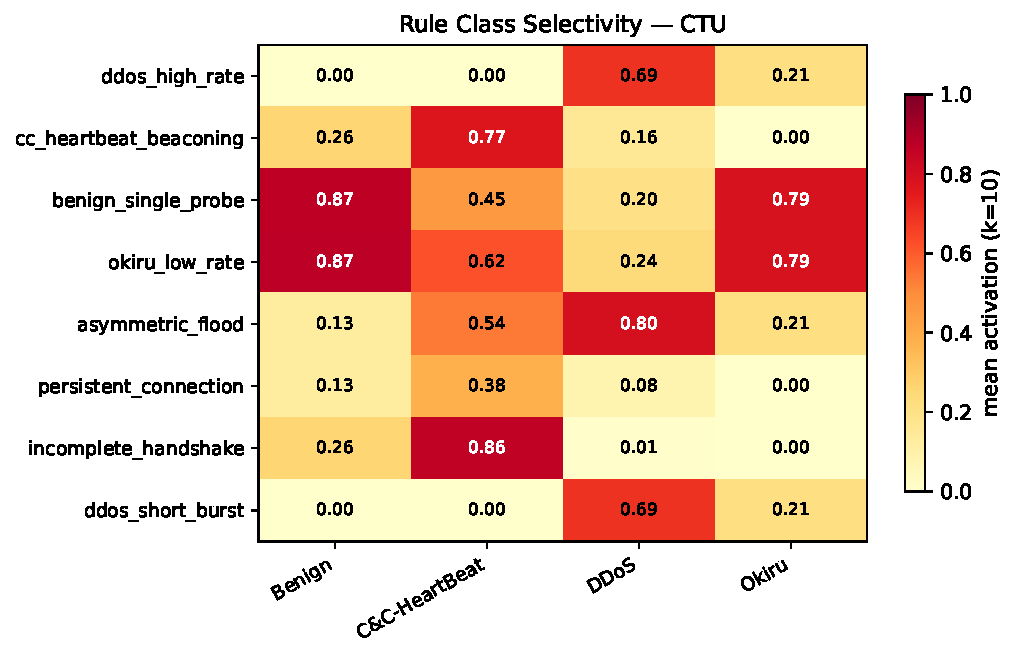
\includegraphics[width=0.47\textwidth,height=5.5cm,keepaspectratio]{figures/rule_selectivity1_ctu.pdf}\hfill
  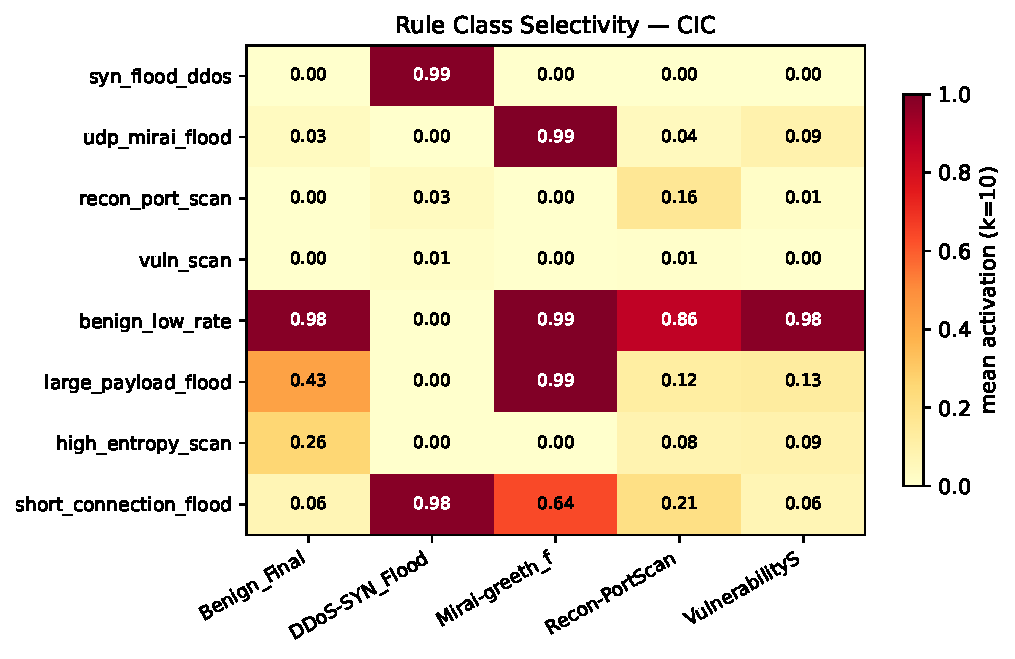
\includegraphics[width=0.47\textwidth,height=5.5cm,keepaspectratio]{figures/rule_selectivity1_cic.pdf}
  \caption{Mean binarised rule activation per known class (seed 0).}
  \label{fig:selectivity}
\end{figure*}

\begin{figure*}[!t]
  \centering
  
\includegraphics[width=0.47\textwidth]{figures/threshold_drift_ctu.pdf}\hfill
  
\includegraphics[width=0.47\textwidth]{figures/threshold_drift_cic.pdf}
  \caption{Per-condition threshold drift (learned $-$ initial), seed~0.
    Red: tightened ($>0$); blue: relaxed ($<0$).}
  \label{fig:threshold_drift}
\end{figure*}

\subsection{The \texorpdfstring{$\alpha$}{alpha}-Gate and Interpretability Trade-Off}
\label{sec:alpha}

We sweep $\lambda_\alpha$ over six values, five seeds each
(Table~\ref{tab:alpha}). The regulariser tunes the gate \emph{monotonically}.
On CTU-IoT-23, $\alpha$ rises from $0.37$ ($\lambda_\alpha{=}0$) to $0.86$
($\lambda_\alpha{=}1.0$); on CIC-IoT-2023, from $0.30$ to $0.95$. An operator
can therefore set rule reliance across most of its range. F1 does not move
($0.9334$--$0.9337$ on CTU, $0.819$--$0.820$ on CIC), and OOD AUROC moves
little and in opposite directions: down by $0.02$ on CTU ($0.911{\to}0.888$)
and up by $0.04$ on CIC ($0.631{\to}0.675$) from $\lambda_\alpha{=}0$ to
$1.0$, in both cases about one to two seed-std. $\lambda_\alpha$ is thus a
control over interpretability with a small OOD side effect rather than a
steep Pareto front (Fig.~\ref{fig:alpha_sweep}). Each point in the sweep was trained
from scratch. Because the penalty acts only on the scalar gate, it should also
be adjustable by fine-tuning a trained model, but we have not tested that.

\begin{table}[t]
\centering\small
\setlength{\tabcolsep}{4pt}
\caption{$\alpha$-gate sweep (NeSy-NIDS, mean over five seeds). $\lambda_\alpha$
monotonically raises the learned gate $\alpha$ (rule reliance) at constant F1;
OOD AUROC drifts down slightly on CTU and up slightly on CIC.}
\label{tab:alpha}
\begin{tabular}{lcccccc}
\toprule
$\lambda_\alpha$ & 0 & 0.05 & 0.1 & 0.2 & 0.5 & 1.0 \\
\midrule
CTU $\alpha$      & 0.37 & 0.54 & 0.68 & 0.79 & 0.84 & 0.86 \\
CTU AUROC         & 0.911 & 0.903 & 0.897 & 0.895 & 0.894 & 0.888 \\
CIC $\alpha$      & 0.30 & 0.80 & 0.85 & 0.90 & 0.93 & 0.95 \\
CIC AUROC         & 0.631 & 0.642 & 0.654 & 0.663 & 0.670 & 0.675 \\
\bottomrule
\end{tabular}
\end{table}

\begin{figure}[t]
  \centering
  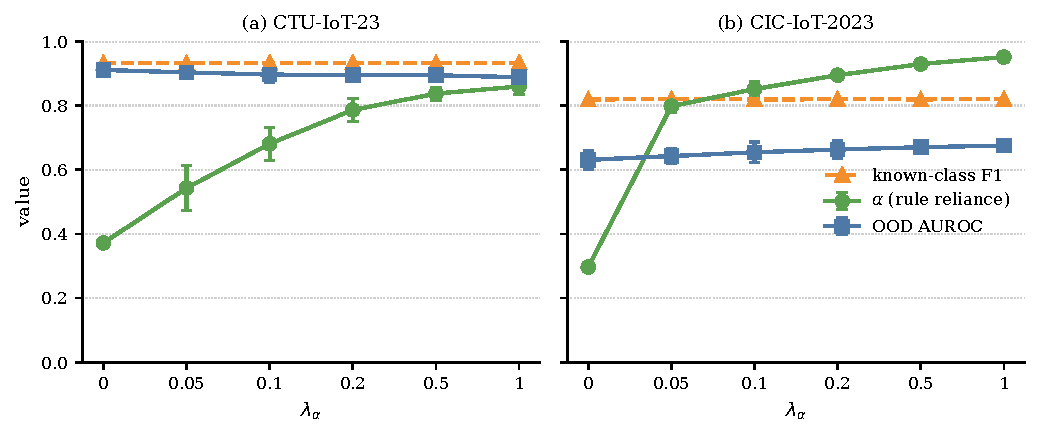
\includegraphics[width=\linewidth]{figures/alpha_sweep.pdf}
  \caption{$\alpha$-gate sweep (NeSy-NIDS, mean over five seeds; error bars
    $\pm$1 std). Raising $\lambda_\alpha$ drives the learned gate $\alpha$
    (rule reliance, green) monotonically upward while known-class F1 (orange,
    dashed) stays flat and OOD AUROC (blue) moves by at most $0.04$: a
    control over interpretability with a small detection side effect rather
    than a steep Pareto front.}
  \label{fig:alpha_sweep}
\end{figure}

\subsection{Concept Leakage and the \texorpdfstring{$\gamma$}{gamma} Ablation}
\label{sec:leakage}

Table~\ref{tab:cbm_concepts} reports mean concept prediction accuracy for
each CBM variant (single seed). JointCBM without concept regularisation
($\gamma{=}0$) reaches 84.9\% on CTU and 92.5\% on CIC. On CTU, accuracy rises
monotonically to 92.7\% at $\gamma{=}1.0$. On CIC it stays at 90--93\% for all
$\gamma$; the \texttt{is\_short\_connection} concept is at 45--52\% in every
variant, a mismatch between its threshold and the z-scored CIC distribution
rather than a regularisation failure. SequentialCBM reaches near-perfect
concept accuracy (99.9\% on CTU, 93.1\% on CIC) because its concept head is
trained on the concept labels alone and frozen before the classifier is
trained. HybridCBM is similar (99.6\% / 92.9\%): its skip connection lets the
classifier bypass the bottleneck, so the concept head is under no
classification pressure and can minimise the BCE loss freely. Higher concept
accuracy means closer agreement with the threshold labels; as the OOD results
show, it does not by itself buy better detection.

\begin{table}[!t]
\renewcommand{\arraystretch}{1.1}
\caption{Mean concept prediction accuracy (\%) per CBM variant (single
seed, indicative; multi-seed $\lambda$ sensitivity in Table~\ref{tab:lambda}).}
\label{tab:cbm_concepts}
\centering
\small
\begin{tabular}{lcc}
\toprule
\textbf{Model} & \textbf{CTU-IoT-23} & \textbf{CIC-IoT-2023} \\
\midrule
JointCBM ($\gamma{=}0$)   & 84.9 & 92.5 \\
JointCBM ($\gamma{=}0.1$) & 86.9 & 91.3 \\
JointCBM ($\gamma{=}0.5$) & 91.8 & 90.2 \\
JointCBM ($\gamma{=}1.0$) & 92.7 & 91.8 \\
SequentialCBM             & 99.9 & 93.1 \\
HybridCBM                 & 99.6 & 92.9 \\
\bottomrule
\end{tabular}
\end{table}

Concept regularisation raises concept \emph{accuracy}: agreement with the
threshold labels climbs from 84.9\% ($\gamma{=}0$) to 92.7\% ($\gamma{=}1.0$)
on CTU-IoT-23 (Table~\ref{tab:cbm_concepts}). Higher accuracy is easily read
as reduced \emph{concept leakage}, but accuracy alone does not measure
leakage. We therefore probe it directly: a linear classifier is trained to
predict the class from (i) the soft concept scores
$\hat{\mathbf{c}}\in[0,1]^K$ and (ii) their binarised values, and leakage is
the accuracy gap, the extra task information carried by the soft deviations
beyond the declared concept values. Leakage is negligible on CTU-IoT-23
(at most $0.002$ for every $\gamma$) and, on CIC-IoT-2023, stays at
$0.05$--$0.08$ with no reliable reduction as $\gamma$ grows ($\gamma{=}0$:
$0.067$; $\gamma{=}0.5$: $0.075$). So $\gamma$ raises concept accuracy but
does not measurably remove leakage and, as Section~\ref{sec:ood} showed,
does not improve open-set detection. Regularisation strength governs concept
accuracy; representation geometry and scorer choice govern OOD detectability
(Table~\ref{tab:scorer}). We accordingly withdraw the earlier claim that
$\gamma$ eliminates concept leakage.

\subsection{Computational Overhead}
\label{sec:compute}

The memory footprint is small. On CTU-IoT-23, JointCBM adds 296 parameters to
the MLP ($+0.3\%$; 93{,}548 vs.\ 93{,}252), and NeSy-NIDS has 13{,}825, about
$7{\times}$ fewer than the MLP (13{,}764 in the neural fallback, the rest in
the rule bank and gate). Both are under $0.4$\,MB in \texttt{float32}. We
report per-flow (batch-1) latency, the conservative regime for a gateway that
scores each flow as it completes. On one thread of an Intel Core i9-9820X,
latency is $96$\,$\mu$s (MLP), $109$\,$\mu$s (JointCBM) and about
$580$\,$\mu$s (NeSy-NIDS, dominated by an un-vectorised per-rule sigmoid loop
that could be batched). These figures come from desktop-class hardware; we
have not measured on ARM gateway processors and make no claim about
on-device performance.


\subsection{Discussion}

\textbf{Representation geometry and scorer choice govern OOD detectability.}
CTU-IoT-23 has four well-separated known classes whose traffic profiles map
cleanly onto the eight expert rules, giving activation clusters with the
covariance structure per-class Mahalanobis exploits. On CIC-IoT-2023 the
rules fire near-deterministically, within-class variance collapses, and
every activation-space scorer fails where a logit-space energy score works
(Table~\ref{tab:scorer}). This adds a qualification to Fort et
al.~\cite{fort2021exploring}: the representation sets the ceiling, and the
scoring rule has to be chosen for the geometry of that representation. The
strength of concept regularisation, by contrast, does not reliably move OOD
AUROC in either direction across ten seeds (Section~\ref{sec:ood}).

\textbf{Inherent vs.\ post-hoc interpretability.}
Post-hoc explainers such as xNIDS~\cite{wei2023xnids} produce faithful
explanations of a black-box model, but the explanation is external to the
model and has to be regenerated, and may change, whenever the model is
retrained. Our architectures carry the interpretable representation inside
the model, at no accuracy cost, and use that same representation for OOD
detection. The two designs serve different needs: a CBM lets an analyst
intervene on concept values at test time, while NeSy-NIDS exposes the learned
thresholds and their drift from the expert specification. Test-time
intervention of this kind is only possible when the interpretable
representation is part of the model~\cite{rudin2019stop}.

\textbf{Deployment implications.}
$\gamma$ and $\lambda_\alpha$ control different things. $\gamma$ raises
concept accuracy but has to be fixed before training, since it shapes the
gradient signal to the encoder. $\lambda_\alpha$ penalises only the scalar
gate $w_\alpha$; in our experiments each $\lambda_\alpha$ setting was trained
from scratch, but nothing in the design prevents adjusting the gate by
fine-tuning a trained model, which we leave to future work. Softmax-based OOD
detectors such as the maximum softmax probability~\cite{hendrycks2017baseline}
and the energy score~\cite{liu2020energy} apply to any classifier but score
in an opaque output space. Our architectures score in the interpretable
bottleneck space (or, on CIC, combine it with the logit space), so a flagged
flow can be \emph{detected} and \emph{diagnosed} from the same concept or
rule activations. Both architectures fit comfortably in the memory and
latency budget of gateway-class hardware measured on a desktop CPU
(Section~\ref{sec:compute}); on-device performance remains to be measured.

\textbf{Limitations.} The main results use five seeds for every learned
model (MLP, CBM variants, NeSy-NIDS), and the CIC $\gamma$ ablation is
replicated on a second independent five-seed set. The alternative-split and
temporal evaluations use three seeds, and Post-hoc~CBM, DT, RF, the post-hoc
OOD baselines and the concept-accuracy table are single runs. Concept and
rule labels are threshold functions written by us, not ground-truth
semantics, so concept accuracy measures agreement with those thresholds.
Per-class Mahalanobis is an approximation on the binary rule-activation
space, which the scorer ablation (Table~\ref{tab:scorer}) addresses directly.
We evaluate two flow-based IoT datasets, one alternative known/unknown split
per dataset and one temporal split (Section~\ref{sec:datasets}); broader
dataset and split coverage, and the test-time intervention that CBMs make
possible, remain future work.

\section{Conclusion}

We evaluated CBMs and NeSy-NIDS as interpretable open-set NIDS on two IoT
datasets under one multi-seed protocol. Both match an unconstrained MLP on
known-class F1 ($\pm0.002$) while exposing a representation an analyst can
read. Open-set detectability is governed by representation geometry and
scorer choice. Per-class Mahalanobis is the best scorer on the well-separated
CTU rule space (NeSy-NIDS $0.911$) but, like every activation-space scorer,
fails on the near-deterministic CIC space ($0.631$), where a logit-space
energy score ($0.728$) restores detection. Concept-fidelity
regularisation strength, in contrast, has no reliable effect on OOD AUROC: a
single-seed ``task-coupling'' effect vanishes and reverses across ten seeds.
Open-set claims about interpretable NIDS need multi-seed replication. Future
work includes data-driven rule and concept discovery, architectures that
combine both bottleneck types, a study of test-time concept intervention, and
evaluation on enterprise-scale traffic with a less favourable
known-to-unknown class ratio.

\section*{Acknowledgment}
The authors declare that no specific funding was received for this research.

\bibliographystyle{IEEEtran}
\bibliography{refs}

\begin{IEEEbiographynophoto}{Crisphine Macharia Ngari}
(Student Member, IEEE) received the B.Sc. degree in Electrical and Computer
Engineering from Gandhi Institute of Technology and Management, India, in 2024. He is currently pursuing the M.Sc degree in Electrical and Computer Engineering with the School of Electrical, Computer and Biomedical Engineering, Southern Illinois University Carbondale. His research interests include machine learning for network security, network intrusion detection systems, interpretable artificial intelligence, open-set recognition for
IoT traffic analysis, and hardware security.
\end{IEEEbiographynophoto}

\begin{IEEEbiographynophoto}{Ning Weng}
(Senior Member, IEEE) received His Ph.D. degree in Electrical and Computer Engineering from
the University of Massachusetts Amherst, Amherst, MA, USA, in 2005.
He is currently a Professor with the School of Electrical, Computer
and Biomedical Engineering, Southern Illinois University-Carbondale, IL, USA.
His research interests include scalable system design for deep packet
inspection, machine learning, network systems, and security.
\end{IEEEbiographynophoto}

\end{document}
